% Nome do capítulo
\chapter{Referencial Teórico}
% Label para referenciar
\label{cap2}

% Diminuir espaçamento entre título e texto
\vspace{-1.9cm}

% Texto do capítulo

    Nesta seção são abordados alguns conceitos e definições importantes para a compreensão do desenvolvimento de aplicações híbridas, alguns componentes que fazem parte do ecossistema mobile e os principais desafios enfrentados por essas tecnologias.
  
\section{A tecnologia \textit{mobile}}

    Assim como em computadores, os dispositivos móveis também possuem diversas opções de sistemas operacionais, dentre elas, os principais são iOS desenvolvido pela \textit{Apple} e Android pelo \textit{Google}. 

    Com a criação dos \textit{smartphones} e \textit{tablets} e a grande quantidade de inovações que estes dispositivos trouxeram junto aos seus sistemas operacionais, os consumidores deixaram de utilizar estes dispositivos somente para ligações ou simples trocas de mensagens, devido a isso, muitas empresas passaram a utilizar deste meio e adaptaram suas necessidades de negócio para gerar conteúdos que atraiam seus clientes, além de prestar serviços de atendimento de maneira rápida e objetiva.
    
    Segundo \citeonline{Galvao2019} esse comportamento do uso do \textit{mobile} é mais do que uma tendência: é uma realidade. Posto que algumas organizações já adaptaram seus processos externos, visando um melhor relacionamento com seus clientes, algumas empresas também tendem a utilizar estas tecnologias visando o ambiente interno. Atualmente, é bastante comum serem usados aplicativos corporativos com foco na otimização de processos e no aperfeiçoamento da comunicação interna \cite{Finzi2019}. A melhoria de processos internos em empresas se faz mais presente no cotidiano das organizações com o avanço do mercado tecnológico e a série de benefícios que estas melhorias podem gerar.

    \subsection{iOS e Android}
      \label{iOS&Android}
      
      Nos últimos anos, o mercado de smartphones tem testemunhado uma batalha entre dois gigantes da tecnologia, a saber, \textit{Apple} e \textit{Google}, empresas responsáveis pelos sistemas operacionais iOS e Android, respectivamente \cite{Cezar2018}. As subseções \ref{iOS} e \ref{Android} apresenta de forma objetiva os principais aspectos de cada sistema operacional afim de contextualizar sobre a representatividade de cada um no meio tecnológico.
      
      \subsubsection{iOS}
       \label{iOS}
       
       O iOS, abreviatura para o nome \textit{iPhone Operation System} é o sistema operacional desenvolvido e mantido pela \textit{Apple}. Em meados de 2007 Steve Jobs apresentou para o mundo o primeiro dispositivo móvel com o sistema iOS, e teve como uma de suas principais características não permitir que o sistema fosse executado em hardware de terceiros, isto é, ele é encontrado somente em aparelhos da própria marca \cite{SARTORELI2018}.
       
       Atualmente, a \textit{Apple} libera versões de atualização geral de seu sistema uma vez por ano, junto ao lançamento de novos dispositivos eletrônicos em grandes eventos organizados pela empresa, são datas esperadas por muitos dos consumidores dos produtos \textit{Apple}, afim de conhecerem os novos produtos e as inovações implementadas no sistema.
      
      \subsubsection{Android}
       \label{Android}
      
      É uma plataforma para tecnologia móvel baseada em uma versão modificada do núcleo \textit{Linux} e de outros \textit{softwares} \textit{open-source}, idealizada por um consórcio de desenvolvedores conhecido como \textit{Open Handset Alliance}(OHA), atualmente o sistema operacional é mantido pelo \textit{Google} no objetivo em conceder uma resposta à crescente demanda da tecnologia móvel no mundo. O Android foi construído com a intenção de permitir aos desenvolvedores criar aplicações móveis que possam tirar total proveito do que um aparelho portátil possa oferecer \cite{pereiraandroid}.
      
      Criado em 2003 pela Android Inc., e vendido ao \textit{Google} em 2005 o que marcou o surgimento do \textit{Google Mobile Division} que fora o primeiro passo para o início da jornada do \textit{Google} no mercado de dispositivos móveis, dois anos depois o Android foi revelado e no ano seguinte lançaram o primeiro dispositivo Android. Na época atual, o Android está presente em grande parte dos recursos inteligentes, como \textit{Smart TV's}, \textit{SmartWatches}, diversos fabricantes de \textit{smartphones} e \textit{tablets}, variantes do Android estão presentes também em \textit{joysticks}, câmeras digitais, computadores entre outros, isso fez com que este sistema se tornasse o mais utilizado em todo o mundo.
      
  \section{Aplicações \textit{mobile}}

  Além das aplicações nativas multiplataformas que são o foco deste trabalho também serão demonstradas as aplicações nativas e híbridas, para que se possa observar as principais diferenças entre as mesmas e identificar em quais contextos melhor se adequa cada tipo de aplicação.

    \subsection{Aplicações nativas}
      \label{app_nativas}
  
    Aplicativos nativos representam uma forma tradicional e comum de desenvolver para dispositivos móveis. Desenvolver uma aplicação nativa exige a prévia definição de um sistema operacional no qual a aplicação poderá ser instalada e executada.
    
    Por ser desenvolvido exclusivamente a um sistema operacional, o código destas aplicações não pode ser reaproveitado no intuito de desenvolver a mesma aplicação para um outro sistema, tornando o desenvolvimento destas aplicações mais custoso, requisitando equipes específicas que dominam a tecnologia a ser utilizada. 
    
    \begin{figure}[h]
    \caption{Ciclo de desenvolvimento de aplicativos nativos}
    \centering % para centralizarmos a figura
    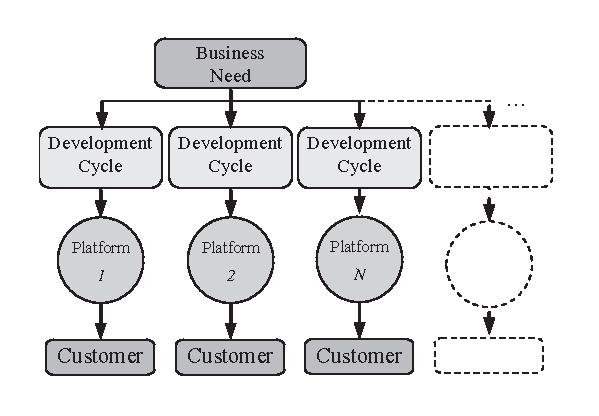
\includegraphics[width=10cm]{imagem/native-development.png}
    \caption*{Fonte: \cite{Corral2012}}
    \label{figura:native-development}
    \end{figure}
    
    Conforme apresentado na figura \ref{figura:native-development}, partindo de uma mesma necessidade de negócio da organização são gerados diferentes ciclos de desenvolvimento com diferentes tecnologias e linguagens para cada plataforma em que o aplicativo poderá ser executado. No Android, por exemplo, é possível utilizar \textit{Java}, \textit{Kotlin} ou C++, no iOS utiliza-se o \textit{Objective-C} ou \textit{Swift} como linguagem de programação.
    
    Existem diversos fatores positivos no desenvolvimento de aplicações nativas. Dado que as aplicações são desenvolvidas exclusivamente para cada ambiente, segue-se os padrões e normas técnicas, de interface e de experiência de usuário determinados pelo sistema, fornecendo uma melhor sensação de aplicação nativa aos usuários. Aplicações nativas têm fácil acesso, por meio de APIs fornecidas pelas plataformas, a recursos dos dispositivos móveis, como sensores, câmera, GPS, contatos e e-mail \cite{S.ElKassas2015}.
    
    \subsection{Aplicações híbridas}
        \label{app_hibridas}
    
    Apesar das vantagens citadas na subseção \ref{app_nativas}, o desenvolvimento de aplicativos nativos para cada sistema operacional pode ser uma alternativa inviável para algumas organizações, por questões relacionadas a custos, maior demanda de recursos técnicos como diferentes equipes de desenvolvimento e conhecimento específico das linguagens de programação de cada plataforma.

    \begin{figure}[h]
    \caption{Ciclo de desenvolvimento de aplicativos híbridos}
    \centering % para centralizarmos a figura
    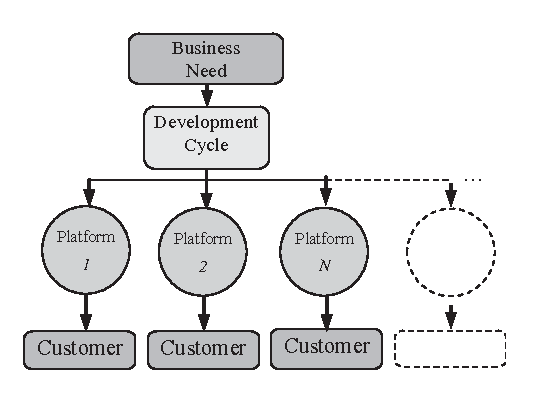
\includegraphics[width=10cm]{imagem/multiplataform-development.png}
    \caption*{Fonte: \cite{Corral2012}}
    \label{figura:multiplataform-development}
    \end{figure}
    
    
    A segunda alternativa para o desenvolvimento de \textit{apps} é a utilização de tecnologias voltadas à \textit{Web} \cite{S.ElKassas2015}. Posto que esta forma de desenvolvimento possibilita a redução de custos, tempo e esforço de desenvolvimento e manutenção do sistema, também exclui a necessidade de múltiplas equipes de desenvolvimento e possibilita a execução da aplicação em diferentes ambientes operacionais. A figura \ref{figura:multiplataform-development} demonstra como é a relação do ciclo de desenvolvimento e a distribuição destas aplicações aos usuários.
    
    \subsection{Aplicações nativas multiplataformas}
        \label{app_multiplataforma_nativa}
    
    São consideradas aplicações nativas multiplataformas, aquelas que a partir de um mesmo código fonte, podem ser instaladas e executadas com código nativo em diferentes sistemas operacionais. Em sua totalidade, este tipo de aplicação reúne todos os pontos positivos das aplicações nativas e hibrídas, explicitados nas subseções \ref{app_nativas} e \ref{app_hibridas}.
    
    \begin{figure}[h]
    \caption{Gráfico comparativo entre \textit{React Native}, \textit{Flutter} e \textit{Xamarin}}
    \centering % para centralizarmos a figura
    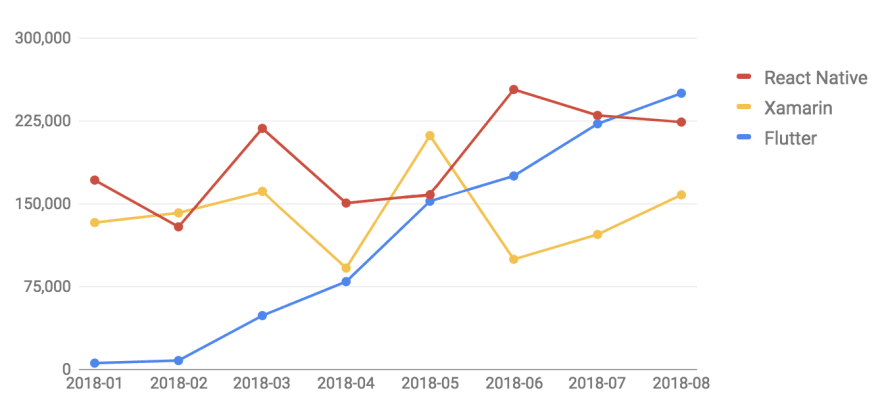
\includegraphics[width=12cm]{imagem/native-frameworks.jpg}
    \caption*{Fonte: \cite{Alferd2019}}
    \label{figura:native-frameworks}
    \end{figure}
    
    \textit{Flutter}, \textit{React Native} e \textit{Xamarin} são os três principais \textit{frameworks} que possibilitam esta abordagem. Na figura \ref{figura:native-frameworks} é apresentado um gráfico do crescimento da utilização destas ferramentas para o desenvolvimento \textit{mobile} ao longo dos anos, considerando a quantidade de aplicativos que utilizam estes \textit{frameworks}. Cada uma destas estruturas tem seus próprios prós e contras, o que dificulta muito realizar um comparativo que defina qual o melhor \textit{framework} a ser utilizado no desenvolvimento, tratando se de uma escolha pessoal e de fato alinhada à real necessidade de negócio na qual a aplicação será envolvida. Para o contexto deste trabalho e da aplicação desenvolvida será tratado com mais profundidade as concepções e particularidades mais relevantes sobre o \textit{React Native} e suas principais bibliotecas para o desenvolvimento.
    
    \section{Desenvolvimento \textit{mobile} nativo multiplataforma}

    De acordo com \citeonline{Corral2012}, aplicações móveis são desenvolvidas de forma dinâmica e lançadas no mercado em pequenos ciclos. Os produtos finais costumam ser de pequeno porte e comercializados a preços baixos. As equipes de desenvolvimento também tendem a ser pequenas. 
    
    Apesar do desenvolvimento \textit{mobile} nativo multiplataforma apresentar se diferentes em alguns pontos, as tradicionais e agéis metodologias e processos de desenvolvimento de software são totalmente aplicáveis neste contexto também, o que poderá diferenciar é apenas as características do produto final.
    
    Esta forma de desenvolvimento obteve um grande crescimento no mercado \textit{mobile} em razão da necessidade de muitas empresas obterem maior produtividade no processo de desenvolvimento junto a criação de aplicações robustas, performáticas e que sejam menos custosas à empresa. \textit{Facebook}, \textit{Instagram}, \textit{Airbnb}, \textit{Nubank} entre outras grandes empresas utilizam essas tecnologias em suas aplicações, com isso é perceptível o quanto essa metodologia de desenvolvimento é referência no mercado.
    
    Dentre as vantagens e diferenças já apresentadas sobre desenvolvimento nativo multiplataforma, pode-se destacar também a facilidade no desenvolvimento pelo fato da utilização de linguagens de programação mais comuns, o que evita a necessidade de um conhecimento aprofundado sobre uma linguagem específica e exclui a necessidade do estudo detalhado de cada plataforma operacional.

    \section{\textit{React Native}}
    \label{react_native}

  \citeonline{Inukollu2014} mostram a possibilidade de desenvolver de forma nativa usando \textit{React Native}, extensão do projeto \textit{React}, originalmente grafado como \textit{ReactJS}.
  
  \textit{React Native} é um \textit{framework} em \textit{JavaScript} para a criação de aplicativos \textit{mobile} reais e nativos para Android e iOS \cite{Eisenman2015}. Como citado, o \textit{React Native} utiliza em seu núcleo o \textit{React}, uma biblioteca em \textit{JavaScript} que se baseia na criação de interfaces através de JSX, uma extensão para o \textit{JavaScript} que possibilita escrever sintaxe XML em meio aos códigos da linguagem, sem qualquer semântica ou delimitação de \textit{tags}, possibilitando escrever a interface junto à lógica de programação.
    
    \subsection{Funcionamento}
    
    De acordo com as definições apresentadas na seção \ref{react_native}, este \textit{framework} grafado em \textit{ReactJS}, trabalha também com Virtual DOM para a renderização de suas interfaces. O DOM(\textit{Document Object Model}) é uma árvore composta de elementos gráficos em uma página e devido a sua estrutura, algumas mudanças destes elementos tendem a afetar em questões e performance e usabilidade das aplicações, porém o \textit{React} trabalha somente com a atualização do Virtual DOM de cada componente renderizado, buscando por alterações nos mesmos, comparando o estado do Virtual DOM com uma imagem do DOM feita antes das alterações e identificando o que realmente foi alterado para o incremento somente deste componente. É possível verificar este fluxo na figura \ref{figura:virtual-dom} abaixo.
    
    \clearpage
    
    \begin{figure}[h]
    \caption{Virtual DOM no React Native}
    \centering % para centralizarmos a figura
    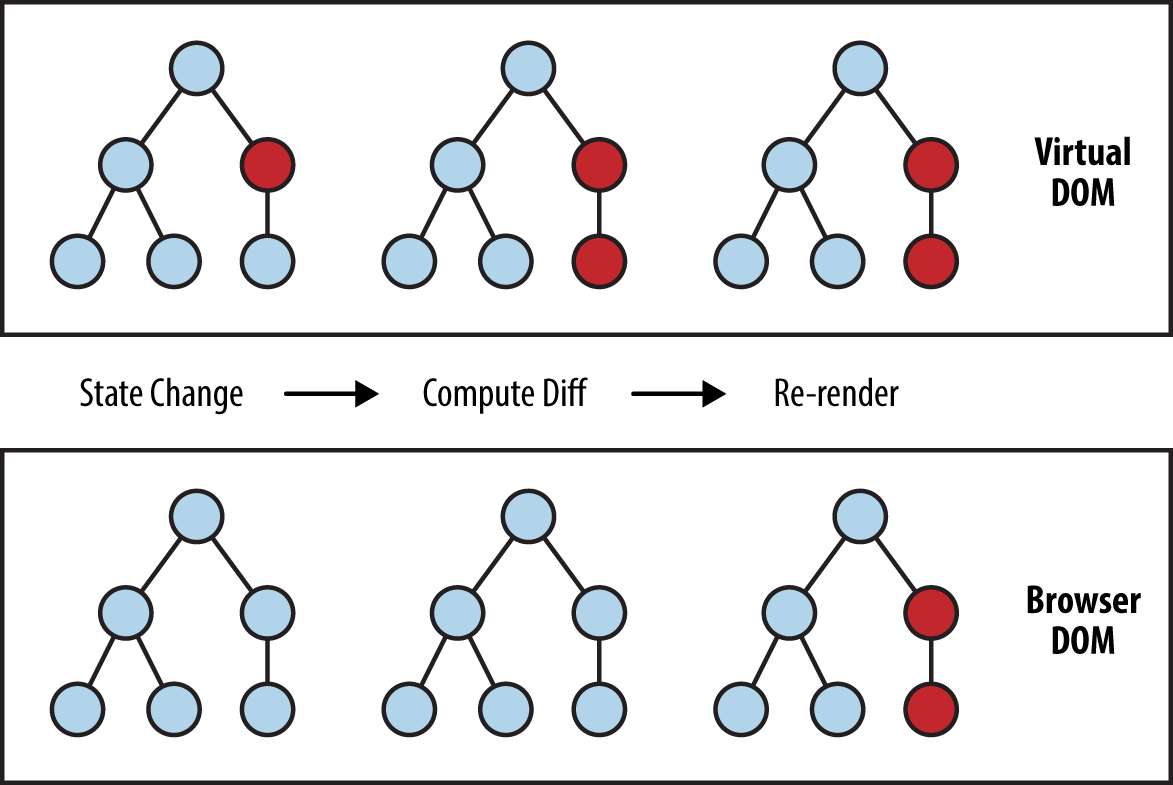
\includegraphics[width=10cm]{imagem/virtual-dom.png}
    \caption*{Fonte: \cite{Eisenman2016}}
    \label{figura:virtual-dom}
    \end{figure}
    
    Mesmo possuindo uma sintaxe semelhante à do \textit{ReactJS} por também utilizar o JSX, existe uma diferença na forma de renderização de seus elementos, conforme indicado na figura \ref{figura:react-native-component}. No React Native, os elementos são emulados de forma nativa, utilizando o \textit{JavaScript Core} que atua como uma ponte entre o JSX e as linguagens. Essa ponte abstrai uma camada de aplicação que possibilita executar API de renderização do \textit{Java}(Android) e do \textit{Objective-C}(iOS).
    
    \begin{figure}[h]
    \caption{Funcionamento da \textit{bridge} no React Native}
    \centering % para centralizarmos a figura
    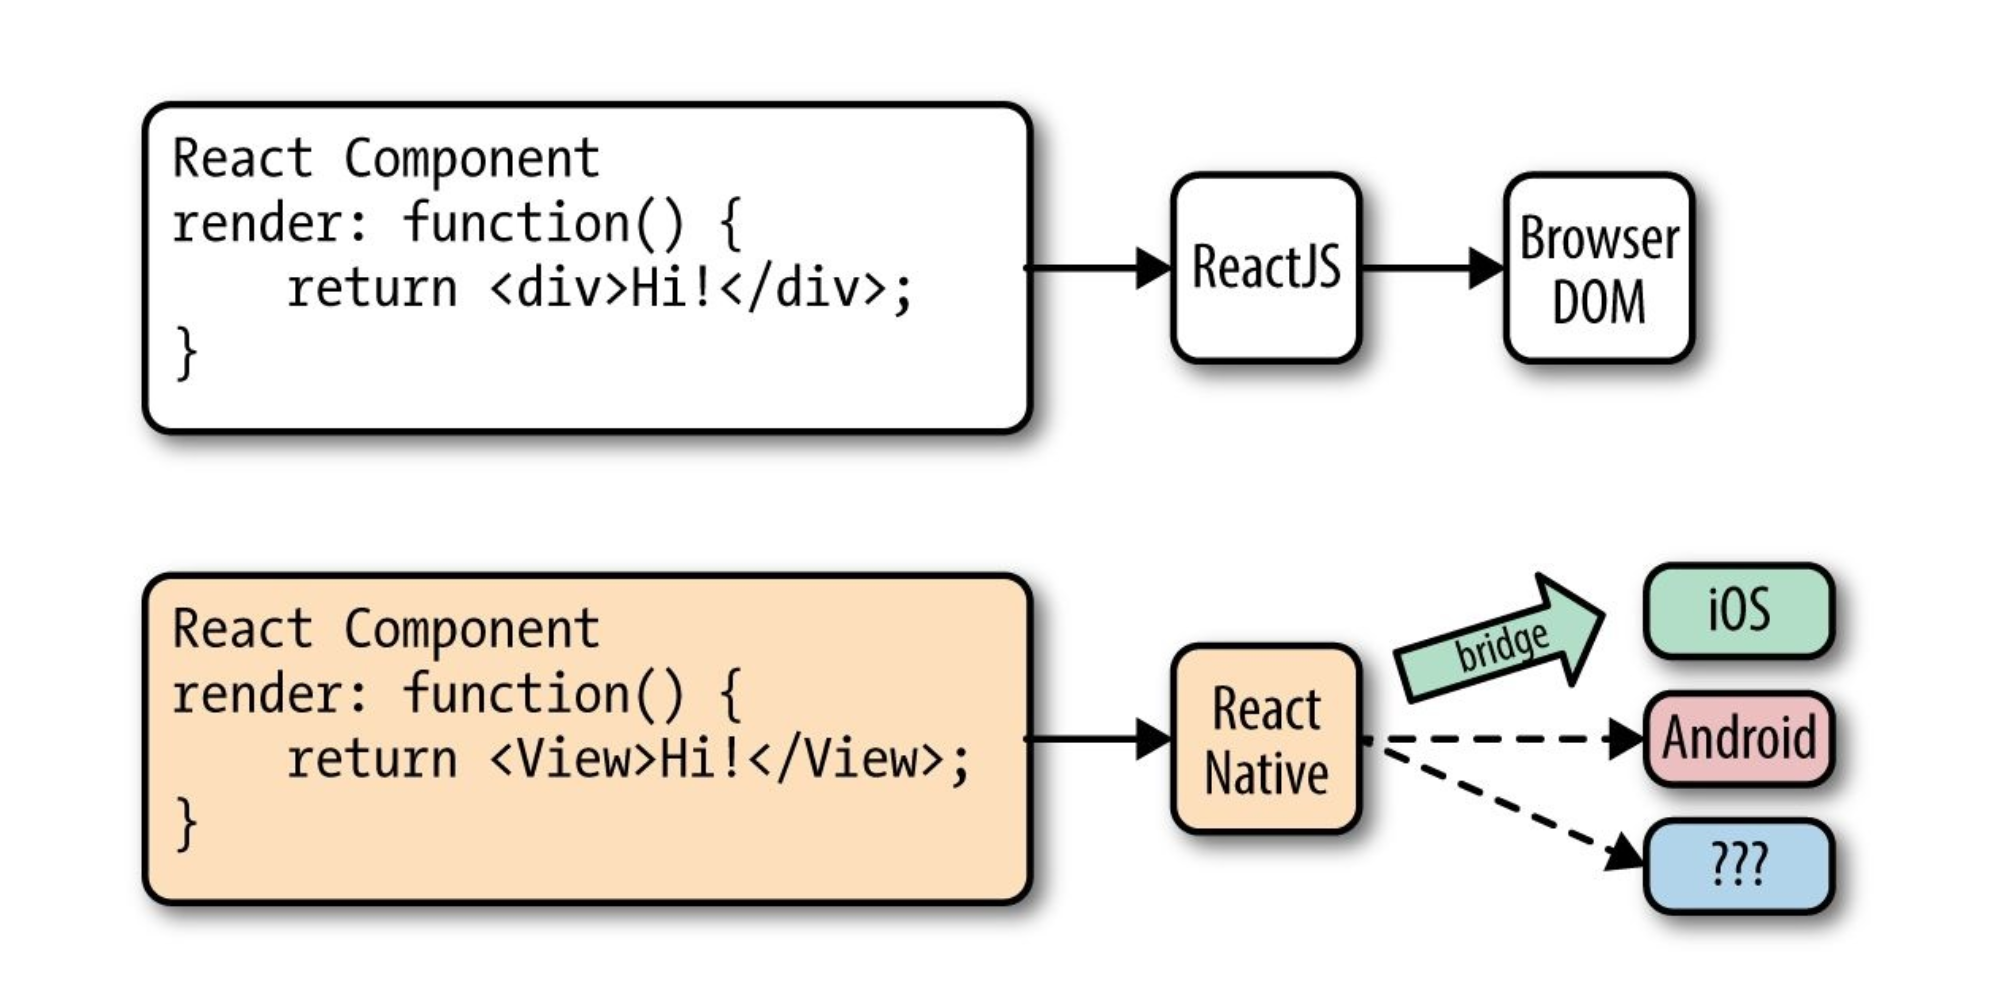
\includegraphics[width=10cm]{imagem/react-native-components.png}
    \caption*{Fonte: \cite{Eisenman2016}.}
    \label{figura:react-native-component}
    \end{figure}
    
    Este \textit{framework} possui três \textit{threads} para executar uma aplicação. A \textit{Shadow Queue}, onde o layout é manipulado; \textit{thread} principal, onde ocorre todo o processo de renderização da interface e a \textit{thread Javascript} onde os \textit{scripts} serão executados \cite{Danielsson998793}.
    
    A orquestração dos componentes nativos de sistema operacional é feita pela "ponte" ~que existe entre o núcleo nativo e o núcleo \textit{JavaScript}. De acordo  com \citeonline{Eisenman2016} Eisenman(2016,  p.  17), \begin{quote} [...] \textit{React  Native} invoca  as  APIs de renderização nativas em \textit{Objective-C} (para iOS) ou \textit{Java} (para Android), além disso ele transpila, minifica e otimiza um código feito em \textit{JavaScript} pelo seu próprio \textit{bundler} chamado \textit{Metro}. \end{quote}
    
    \subsection{Arquitetura}
    \label{react_native_mvp}
    
    Por sua clareza em termos de código, facilidade ao implementar testes automatizados e economia no tempo inicial da estruturação de um aplicativo, o MVP (\textit{Model-View-Presenter}) é um dos padrões mais adotados em aplicações \textit{React Native} e o seu fluxo de informações e troca de mensagens é representado abaixo na figura \ref{figura:react-native-mvp}.
    
    \begin{figure}[h]
    \caption{Fluxo de informações no MVP}
    \centering % para centralizarmos a figura
    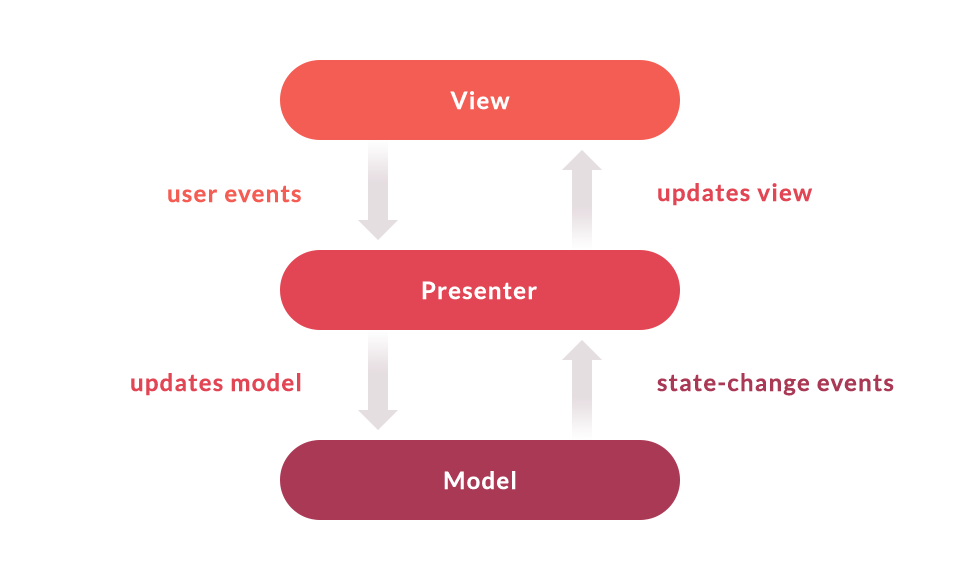
\includegraphics[width=12cm]{imagem/react-mvp.png}
    \caption*{Fonte: \cite{Teles2017}}
    \label{figura:react-native-mvp}
    \end{figure}
    
    O Model-View-Presenter é um padrão arquitetural derivado do MVC (\textit{Model-View-Controller}), a principal diferença é que no MVC o \textit{model} dispara atualizações ao \textit{view} sendo essas atualizações intermediadas pelo \textit{controller}, no MVP quem realiza essas intermediações é a camada \textit{presenter} sendo a principal responsabilidade deste componente, controlar o que será exibido ao \textit{view}, enquanto o \textit{view} é encarregado de organizar estes elementos para exibição ao usuário e o \textit{model} possui as mesmas atribuições que no padrão MVC.
    
    \section{Ferramentas e bibliotecas para o desenvolvimento em \textit{React Native}}
    \label{ferramentas-react-native}
    
    O objetivo desta seção é destacar e apresentar as definições das principais ferramentas e bibliotecas utilizadas no desenvolvimento do aplicativo para o laboratório de audiovisual e fotografia da PUC MINAS.
    
    \subsection{Expo}
    O Expo é uma ferramenta utilizada no desenvolvimento mobile com React Native que permite o fácil acesso às API’s nativas do dispositivo sem precisar instalar qualquer dependência ou alterar código nativo \cite{Fernandes2018}. Além disto, essa ferramenta possibilita o desenvolvimento sem a necessidade de instalar a SDK do Android e do XCode para Mac, possibilitando também a execução das versões de desenvolvimento do aplicativo em um dispositivo móvel que possui instalado o aplicativo Expo afim de testar e verificar o comportamento da aplicação na plataforma operacional.
    
    \subsection{React Navigation}
    É composto por alguns utilitários que criam uma estrutura de navegação em aplicativos \textit{React Native}. O React Navigation foi lançado em 2018 e é a biblioteca de navegação do \textit{React Native}, responsável por orquestrar todo o roteamento e navegação entre telas da aplicação de maneira simples e robusta.
    
    \subsection{Axios}
    Apesar de seu uso não ser exclusivamente do \textit{React Native}, o Axios é uma biblioteca que faz parte de todo o ecossistema \textit{JavaScript}, feita para realizar requisições HTTP baseando se no conceito de promises e é muito utilizada para consumir API's no intuito de buscar informações necessárias as aplicações.
    
    \subsection{ESLint}
    O ESLint é uma ferramenta utilizada para identificar e relatar padrões encontrados no código \textit{ECMAScript} / \textit{JavaScript}, com o objetivo de tornar-lo mais legível e consistente evitando possíveis problemas na codificação, antes de sua execução. Sua utilização é muito importante para padronizar espaçamentos e identações em todos os trechos de código da aplicação.
  
      
    \section{Aplicações correlatas}
    
    \subsection{GimmeBack}
    
    O GimmeBack é um aplicativo que permite aos usuários cadastrarem objetos que serão disponibilizados para empréstimo a terceiros e programarem a data para devolução do mesmo, além de contar com um sistema de alertas e notificações para recordar os usuários sobre os prazos.
    
    \begin{figure}[h]
    \caption{Tela de empréstimos ativos}
    \centering % para centralizarmos a figura
    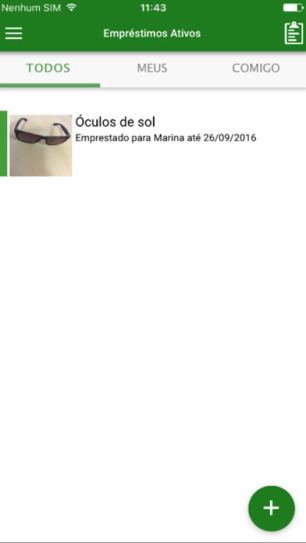
\includegraphics[width=8cm]{imagem/gimmeback-img.jpeg}
    \caption*{Fonte: \cite{MOBILE2016}}
    \label{figura:gimmeback}
    \end{figure}
    
    \subsection{Peerby}
    
    É um sistema que facilita o empréstimo de objetos entre pessoas que moram até 30 minutos de distância, funcional somente na Holanda, essa ferramenta tem como objetivo diminuir compras de coisas que são necessárias em poucos momentos, criando uma ideia mais sustentável de consumo. Em funcionalidades, o solicitante cadastra o objeto que está procurando, enquanto os demais usuários que possuírem aquele item, entram na solicitação e alertam o solicitante sobre a disponibilidade de realizar o empréstimo, um fluxo inverso se comparado ao GimmeBack e o aplicativo do laboratório.
    
    \begin{figure}[h]
    \caption{Tela de vizinhos próximos}
    \centering % para centralizarmos a figura
    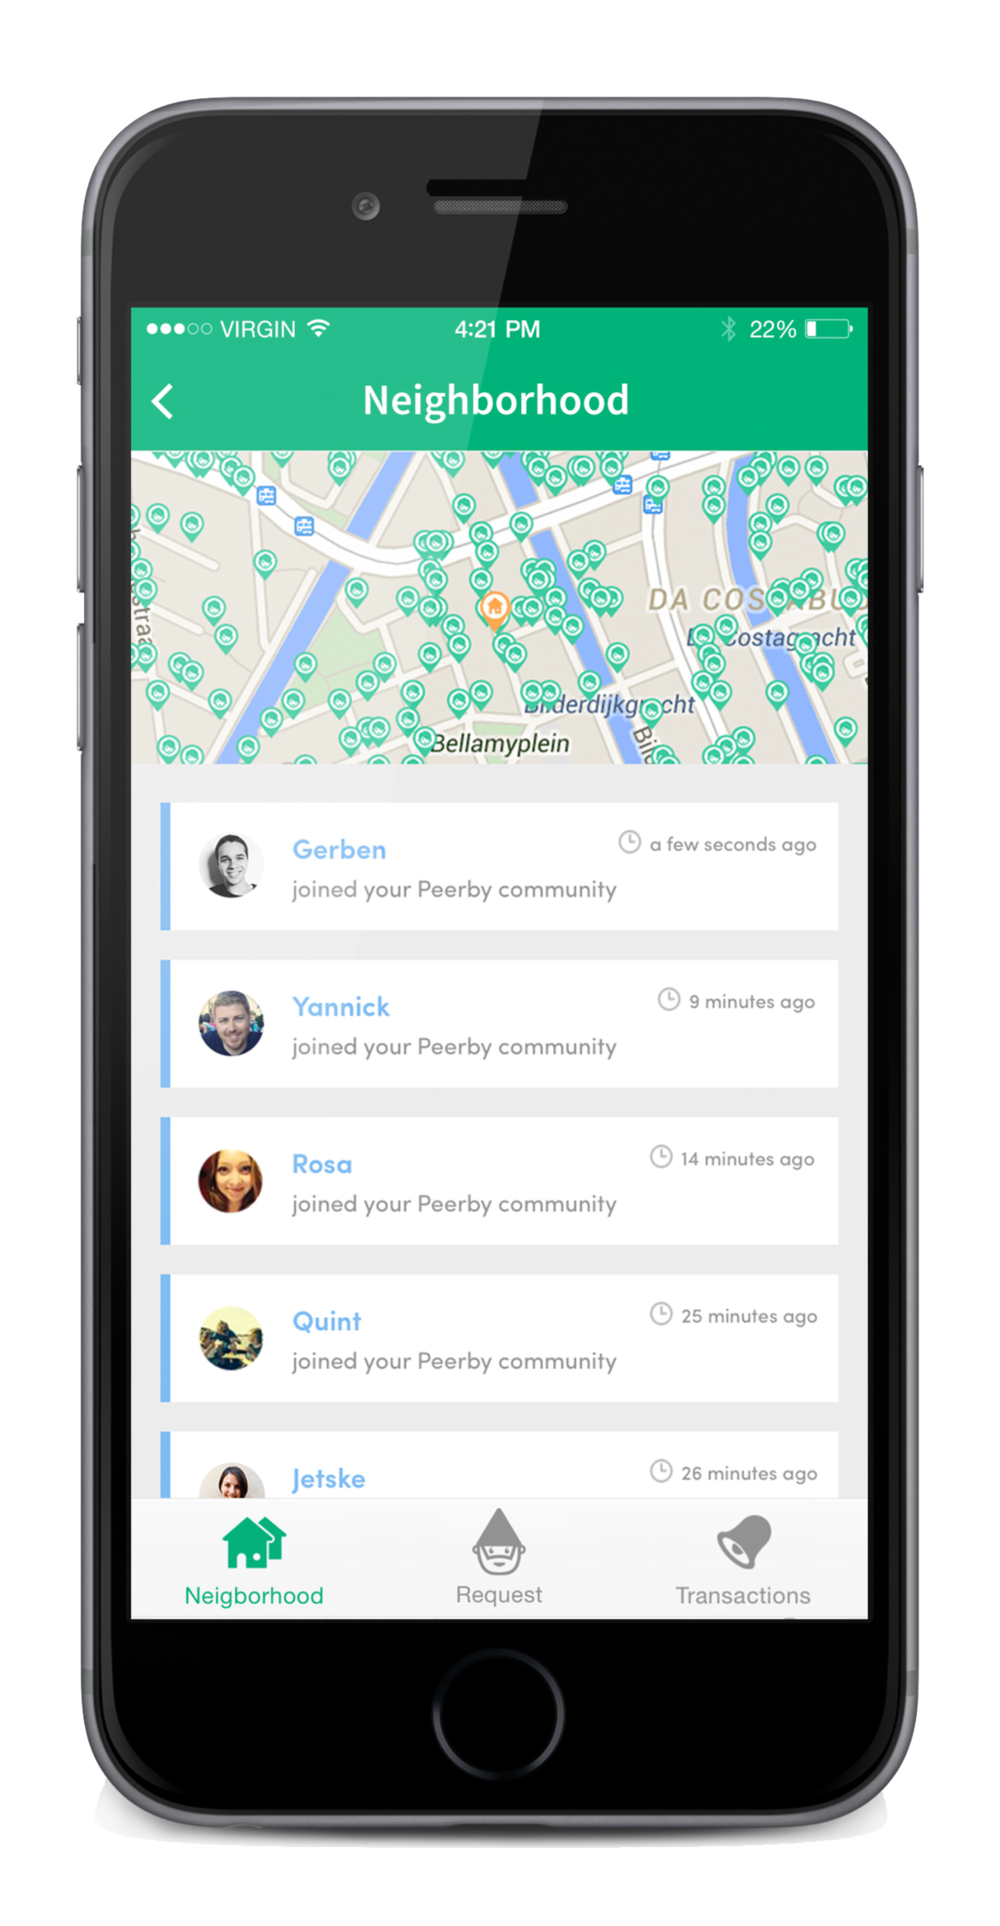
\includegraphics[width=8cm]{imagem/peerby-img.png}
    \caption*{Fonte: \cite{PEERBY2014}}
    \label{figura:peerby}
    \end{figure}
    
    \subsection{Tem açucar?}
    
    Seguindo a mesma linha do Peerby, o aplicativo Tem açucar? foi criado com o objetivo de promover o compartilhamento de objetos com vizinhos, de modo sustentável e que promova uma boa relação entre os mesmos. Portanto é possível buscar por objetos a serem emprestados pela plataforma, avaliar a experiência de empréstimo e ter acesso a esses objetos de forma mais simples e segura.
    
    \begin{figure}[h]
    \caption{Tela de solicitação}
    \centering % para centralizarmos a figura
    \includegraphics[width=8cm]{imagem/temaçucar-img.jpg}
    \caption*{Fonte: \cite{NATALIA2020}}
    \label{figura:comparative-board}
    \end{figure}
    
    \subsection{Comparativo}
    
    Além do quadro comparativo abaixo, é importante destacar o propósito e o público alvo de cada aplicativo citado anteriormente. Começando pelo GimmeBack que tem o objetivo de tornar se uma comunidade de compartilhamento de objetos sem com que as pessoas tenham dificuldades em emprestar e receber de volta seus itens, atualmente o aplicativo é utilizado até por algumas bibliotecas escolares para organizar melhor o empréstimo de livros a alunos. Em seguida, apesar de ainda não funcionar no Brasil, o aplicativo Peerby busca influenciar boas práticas conectando vizinhos ou pessoas de um mesmo bairro para que os mesmo compartilhem seus pertences entre si, socializando as ideias e necessidades cotidianas e o aplicativo Tem Açucar? propõe a ideia de uma rede social de vizinhos que facilite a comunicação, colaboração e troca de gentilezas nas vizinhanças. Em contra ponto, o aplicativo desenvolvido para o laboratório de audiovisual e fotografia da PUC MINAS, apesar de compartilhar algumas semelhanças em termos de funcionalidade e ideia central, tem seu público alvo focado nos alunos da universidade com um nicho pré definido de objetos/equipamentos que irão compor os cenários dos empréstimos.
    
    \begin{figure}[h]
    \caption{Quadro comparativo}
    \centering % para centralizarmos a figura
    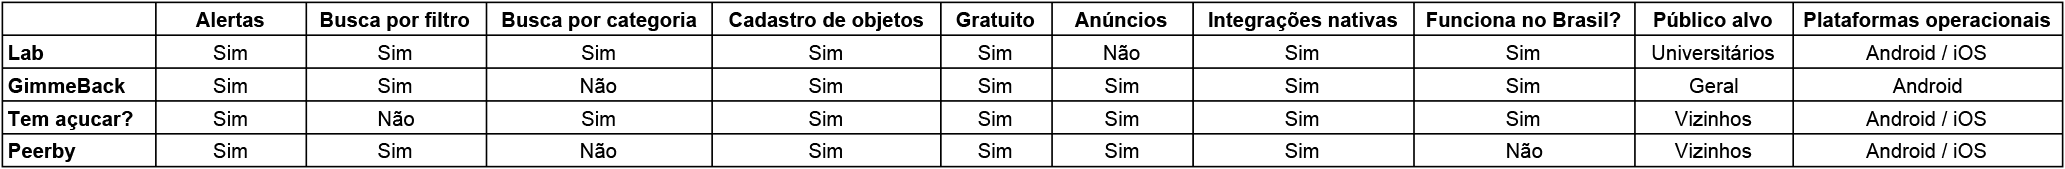
\includegraphics[width=16cm]{imagem/quadro-comparativo.png}
    \caption*{Fonte: Autor}
    \label{figura:comparative-board}
    \end{figure}
